\section{Image display}
The intention was to rotate the motor at a given speed, such that POV would occurs. POV also called persistence of vision, is the phenomenon that states that the human eye  
always retains images for a fraction of a second (around 0.04 second). \todo[inline]{ref til \url{http://www.mediacollege.com/glossary/p/persistence-of-vision.html}}. 

\todo[inline]{image... Image in a raster grid}
The image that had to be displayed, was drawn in a raster grid. Using the encoders , would it be  possible to provide some form of information of the angular position of the LED strips, and thereby which pixels had to be displayed. 

\todo[inline]{image in raster grid , and the propellor placed in angle..}

A problem faced here was on how to determine which pixel had to be displayed, in a discrete image description. The problem here is given an angle and a endpoint on how to draw a straight line within these two points, and how to determine the in between pixel positions. \\
Finding the endpoint and angle was pretty easy, the angle was given by the encoders, and the endpoint could easily be calculated trig identities. \\

To draw the line between two points (being the startpoint and the endpoint) were an modified version of Bresenham line algorithm used,  modified as the original algorithm is only capable of handling cases from where the slope between the two points is between 0 and 1. \\

The Bresenham line algorithm is an algorithm used for determining the in between points in raster grid.  It compares 

\begin{figure}[H]
	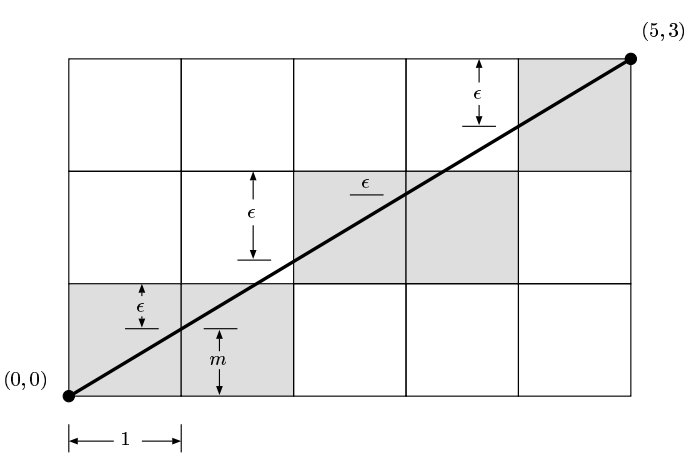
\includegraphics[width = \textwidth]{images/bresenham}
	\caption{Bresenham line algorithm applied on a simple case}
	\label{fig:bresenham_line}
\end{figure}
\todo[inline]{http://www.idav.ucdavis.edu/education/GraphicsNotes/Bresenhams-Algorithm.pdf}
It keeps track of an error value being $\epsilon$ , which represent the distance real line to the top edge of the pixel. 
 
%This means that everything we see is a subtle blend of what is happening now and what happened a fraction of a second ago.

